\documentclass[tikz,border=4pt]{standalone}
\usetikzlibrary{arrows.meta}

\begin{document}
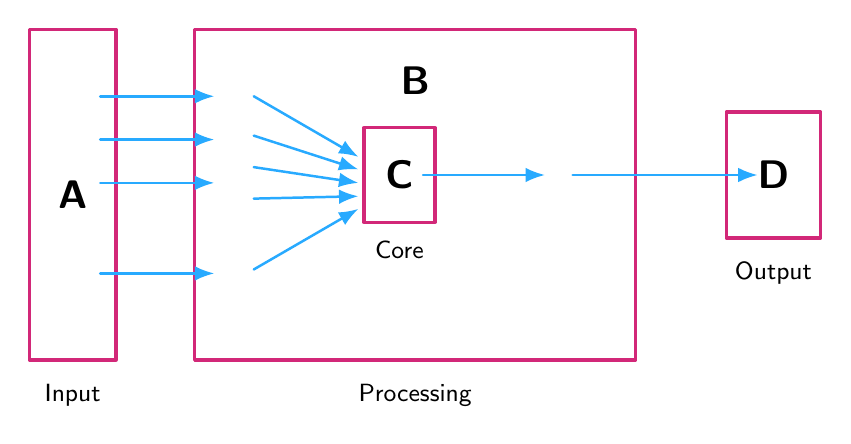
\begin{tikzpicture}[x=1cm,y=1cm,>=Latex,line cap=round,line join=round]

% Colors
\definecolor{boxpink}{RGB}{210,40,120}
\definecolor{arrowblue}{RGB}{40,170,255}

% Text styles
\tikzset{
  boxlabel/.style={font=\sffamily\bfseries\Large},
  boxcaption/.style={font=\sffamily\small,align=center}
}

% Left tall box
\draw[draw=boxpink,line width=1.2pt] (0,0) rectangle (1.1,4.2);

% Large middle box
\draw[draw=boxpink,line width=1.2pt] (2.1,0) rectangle (7.7,4.2);

% Small inner middle box
\draw[draw=boxpink,line width=1.2pt] (4.25,1.75) rectangle (5.15,2.95);

% Right box
\draw[draw=boxpink,line width=1.2pt] (8.85,1.55) rectangle (10.05,3.15);

% Box labels
\node[boxlabel] at (0.55,2.1) {A};
\node[boxlabel] at (4.9,3.55) {B};
\node[boxlabel] at (4.7,2.35) {C};
\node[boxlabel] at (9.45,2.35) {D};

% Captions below boxes
\node[boxcaption] at (0.55,-0.45) {Input};
\node[boxcaption] at (4.9,-0.45) {Processing};
\node[boxcaption] at (4.7,1.4) {Core};
\node[boxcaption] at (9.45,1.1) {Output};

% Four horizontal arrows from left box to middle box
\foreach \yy in {3.35,2.8,2.25,1.1} {
  \draw[draw=arrowblue,line width=0.9pt,->] (0.9,\yy) -- (2.35,\yy);
}

% Five converging arrows inside middle box toward inner box
\draw[draw=arrowblue,line width=0.9pt,->] (2.85,3.35) -- (4.18,2.58);
\draw[draw=arrowblue,line width=0.9pt,->] (2.85,2.85) -- (4.18,2.42);
\draw[draw=arrowblue,line width=0.9pt,->] (2.85,2.45) -- (4.18,2.25);
\draw[draw=arrowblue,line width=0.9pt,->] (2.85,2.05) -- (4.18,2.08);
\draw[draw=arrowblue,line width=0.9pt,->] (2.85,1.15) -- (4.18,1.92);

% Arrow from inner box to right side of middle box
\draw[draw=arrowblue,line width=0.9pt,->] (5.0,2.35) -- (6.55,2.35);

% Arrow from middle box to right box
\draw[draw=arrowblue,line width=0.9pt,->] (6.9,2.35) -- (9.25,2.35);

\end{tikzpicture}
\end{document}
